% =====================================================================
%  Appendice A — Le stesse misure sugli altri quattro modelli
%  Inclusa da main.tex dopo \appendix
% =====================================================================

\chapter{Le stesse misure sugli altri modelli}
\label{app:modelli}

Il Capitolo~\ref{cap:risultati1} riporta nel corpo del testo le figure relative
al modello Qwen2.5-3B. Questa appendice raccoglie le corrispondenti figure per
gli altri quattro modelli, organizzate per misura anziché per modello in modo da
rendere immediato il confronto. Gli andamenti sono quelli discussi nel capitolo:
qui interessa mostrare che non dipendono dal modello scelto come esemplare.

Il modello da 14 miliardi di parametri dispone di un solo campione per
temperatura, per cui nelle sue figure le barre d'errore non sono definite e le
curve risultano più irregolari. È la ragione per cui non è stato scelto come
esemplare, nonostante sia il più grande.

% ---------------------------------------------------------------------
\section{Crescita del vocabolario}
\label{app:heaps}

\begin{figure}[!htb]
  \centering
  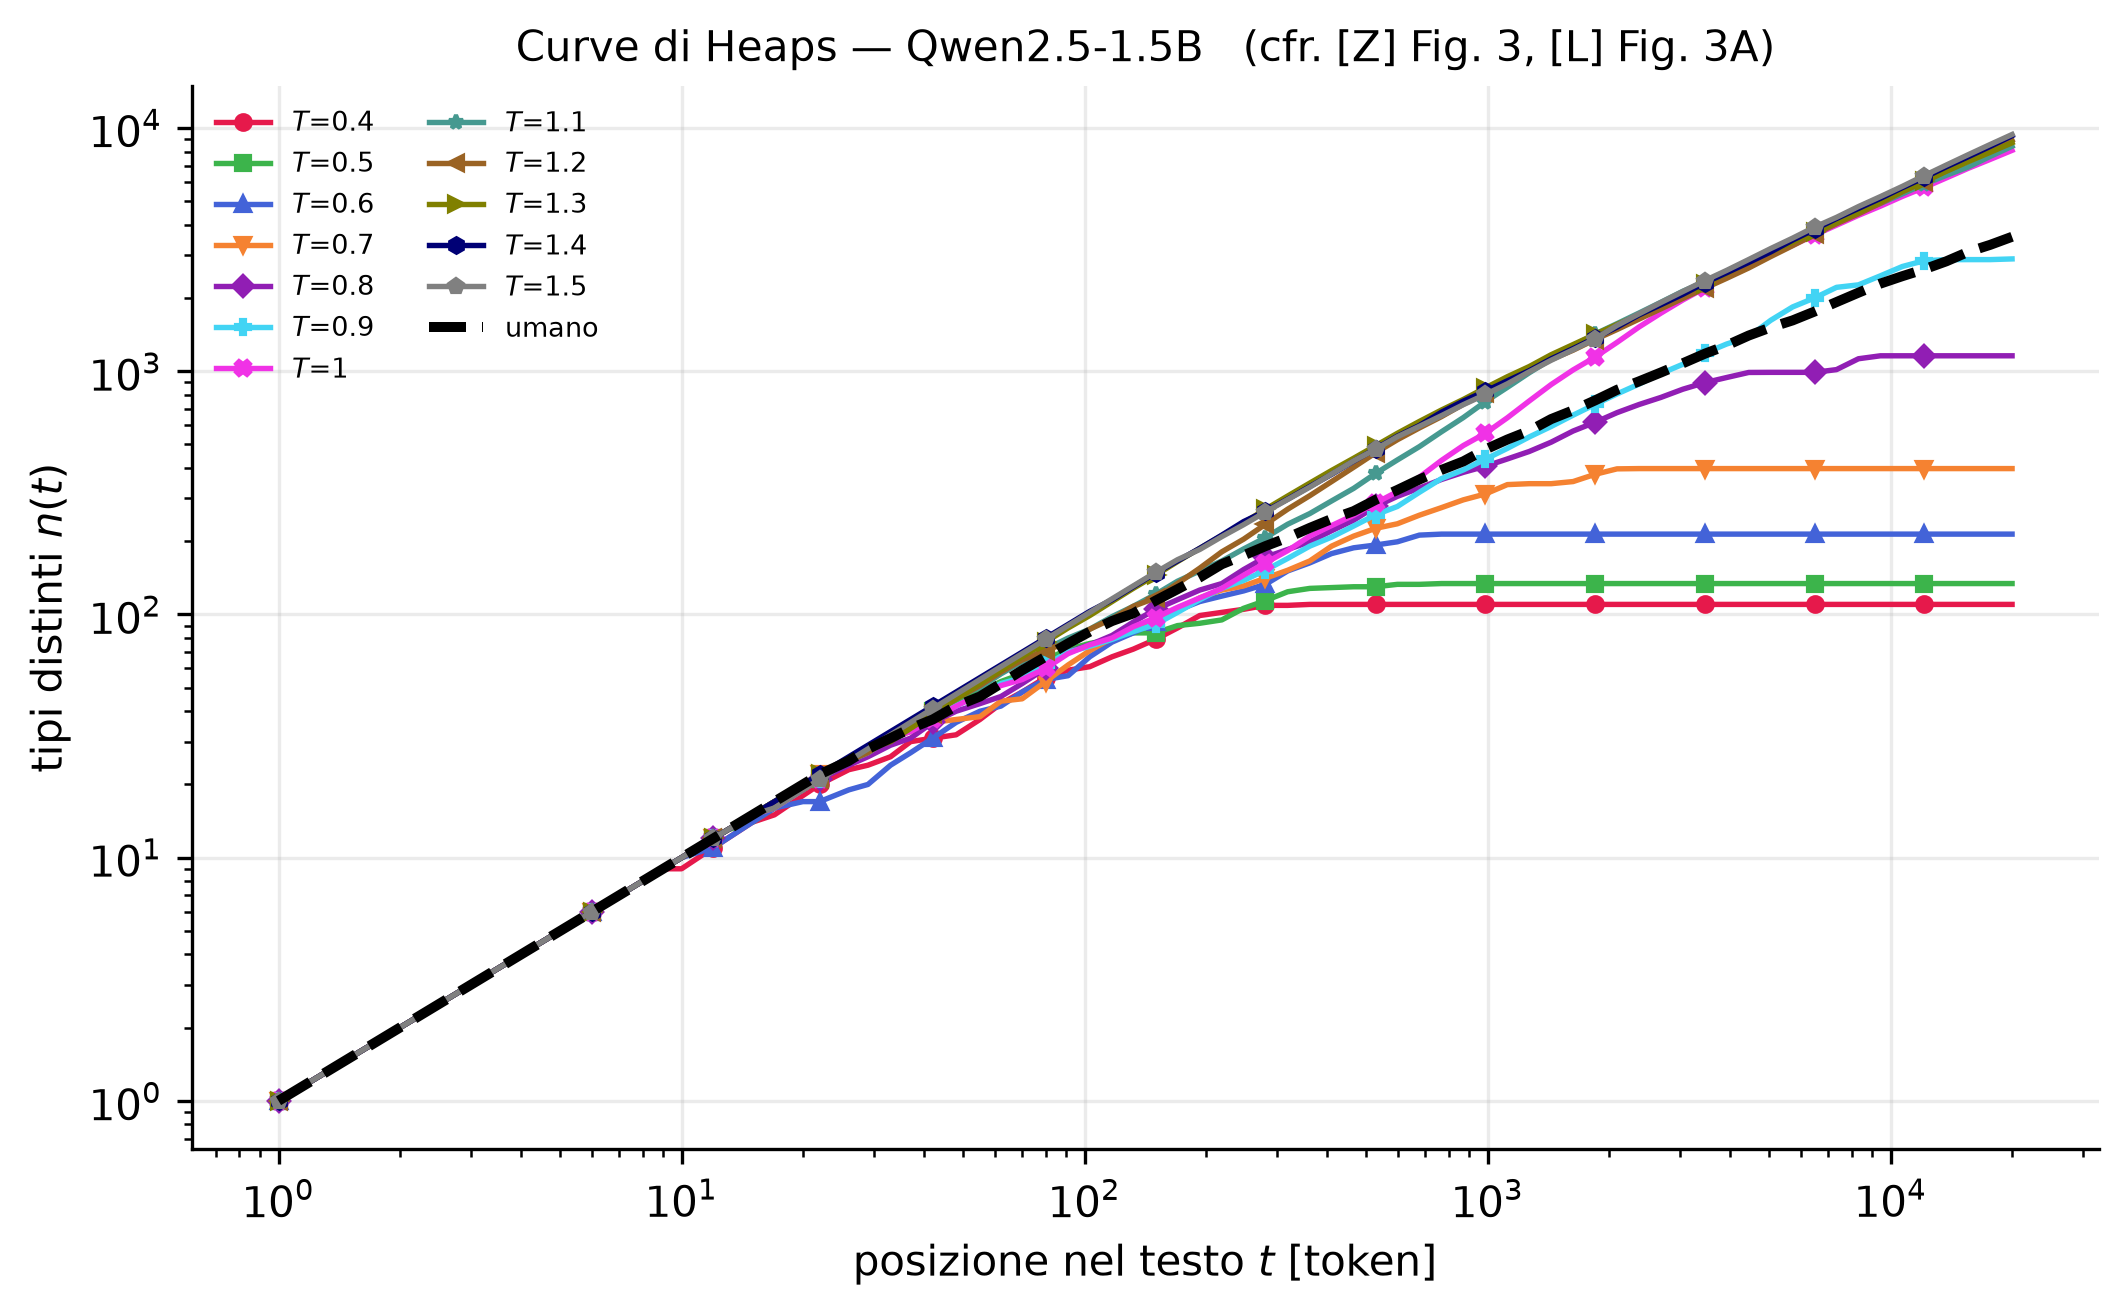
\includegraphics[width=0.56\textwidth]{figure/cap4_heaps_curve_Qwen25_15B.png}
  \caption{Qwen2.5-1.5B.}
\end{figure}

\begin{figure}[!htb]
  \centering
  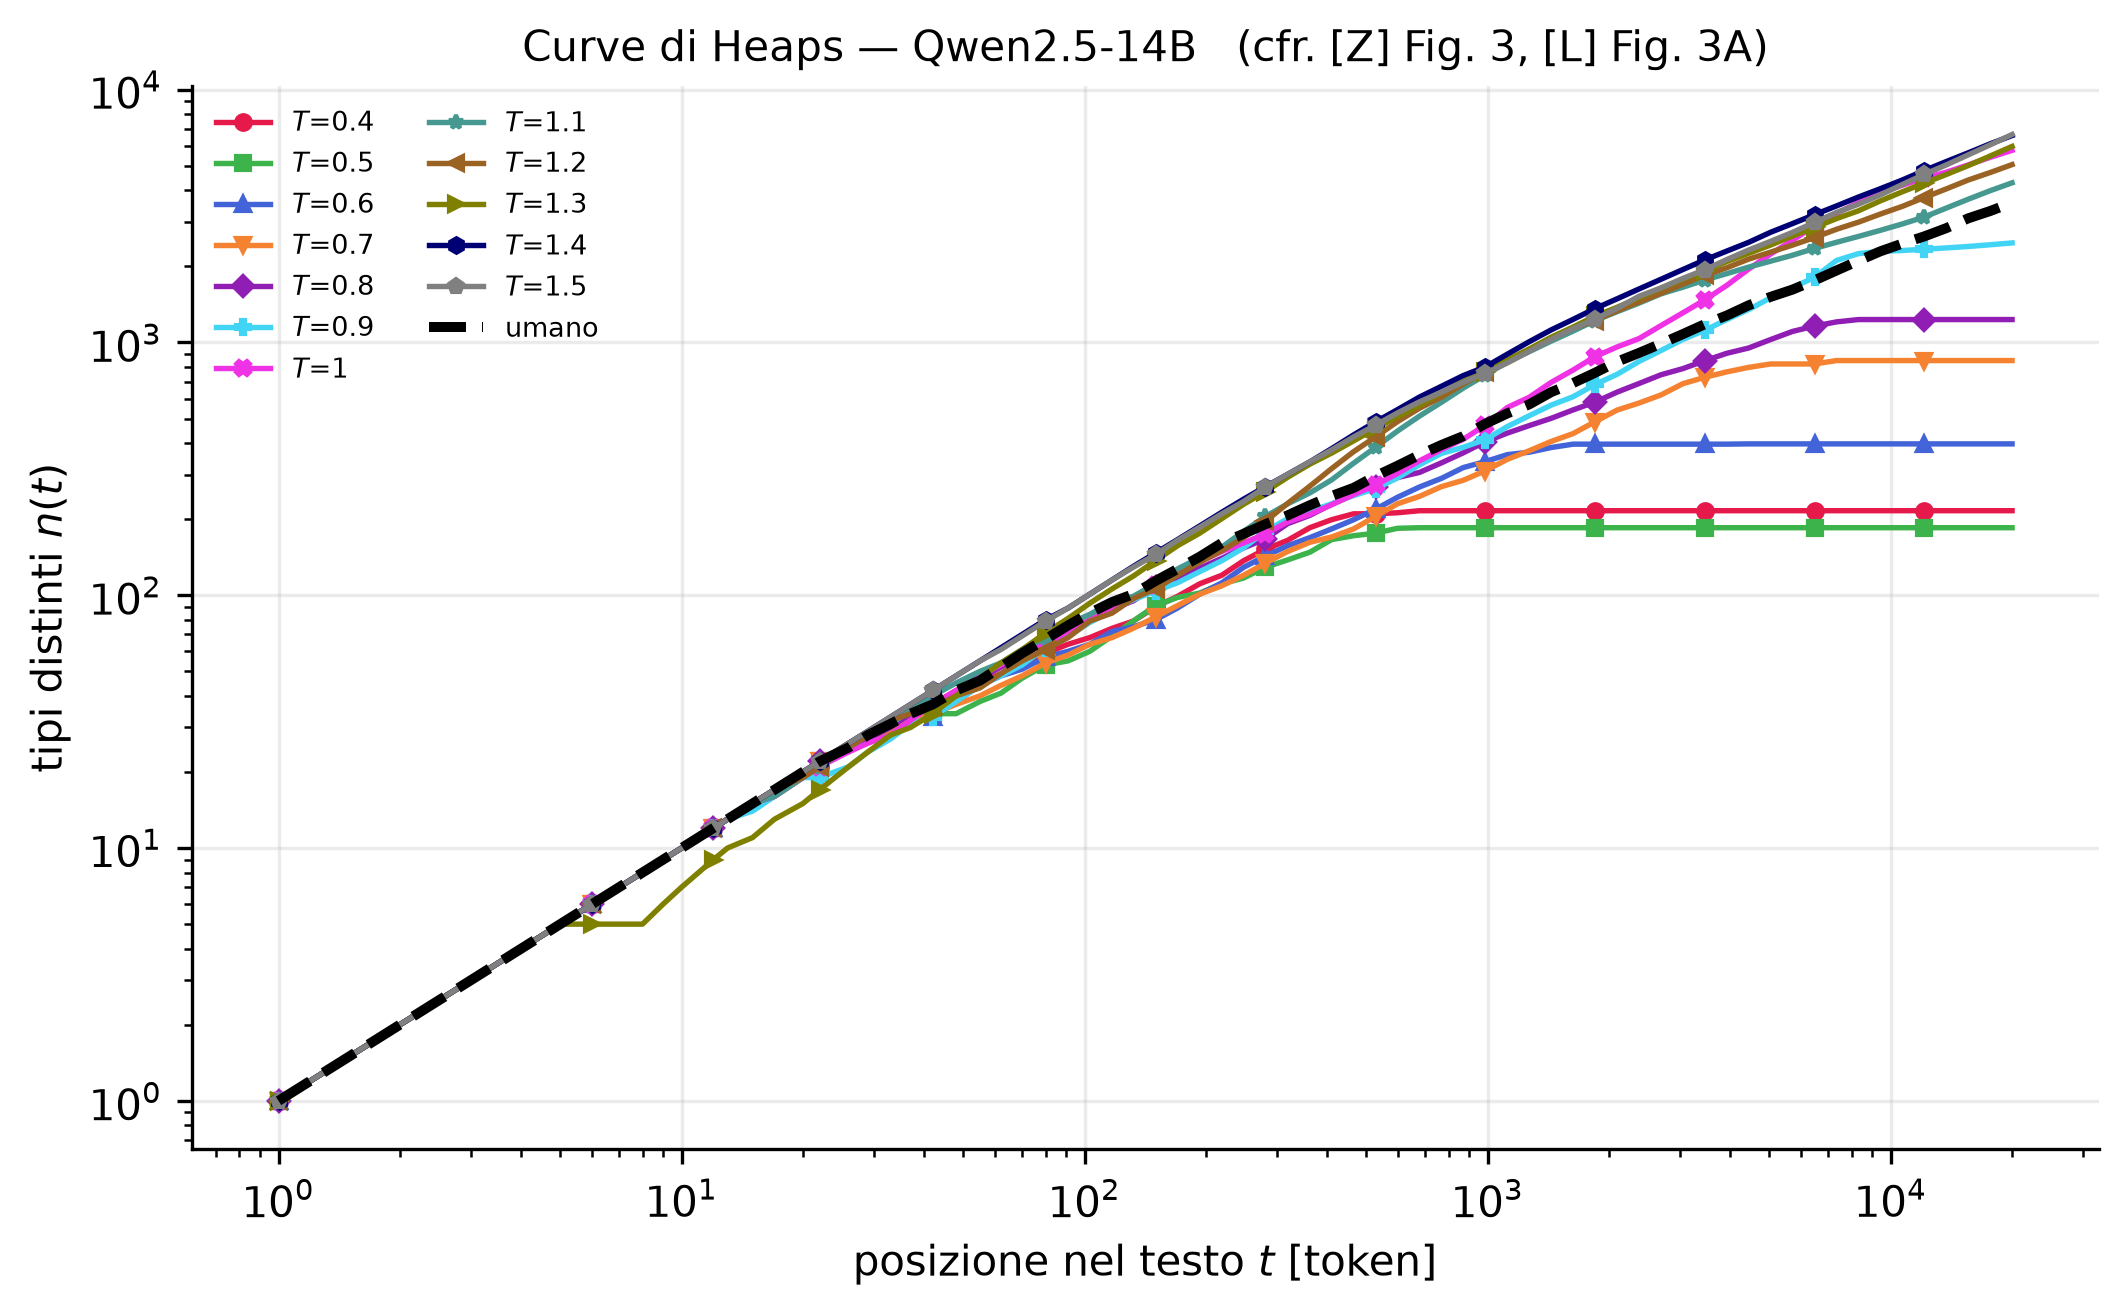
\includegraphics[width=0.56\textwidth]{figure/cap4_heaps_curve_Qwen25_14B.png}
  \caption{Qwen2.5-14B.}
\end{figure}

\begin{figure}[!htb]
  \centering
  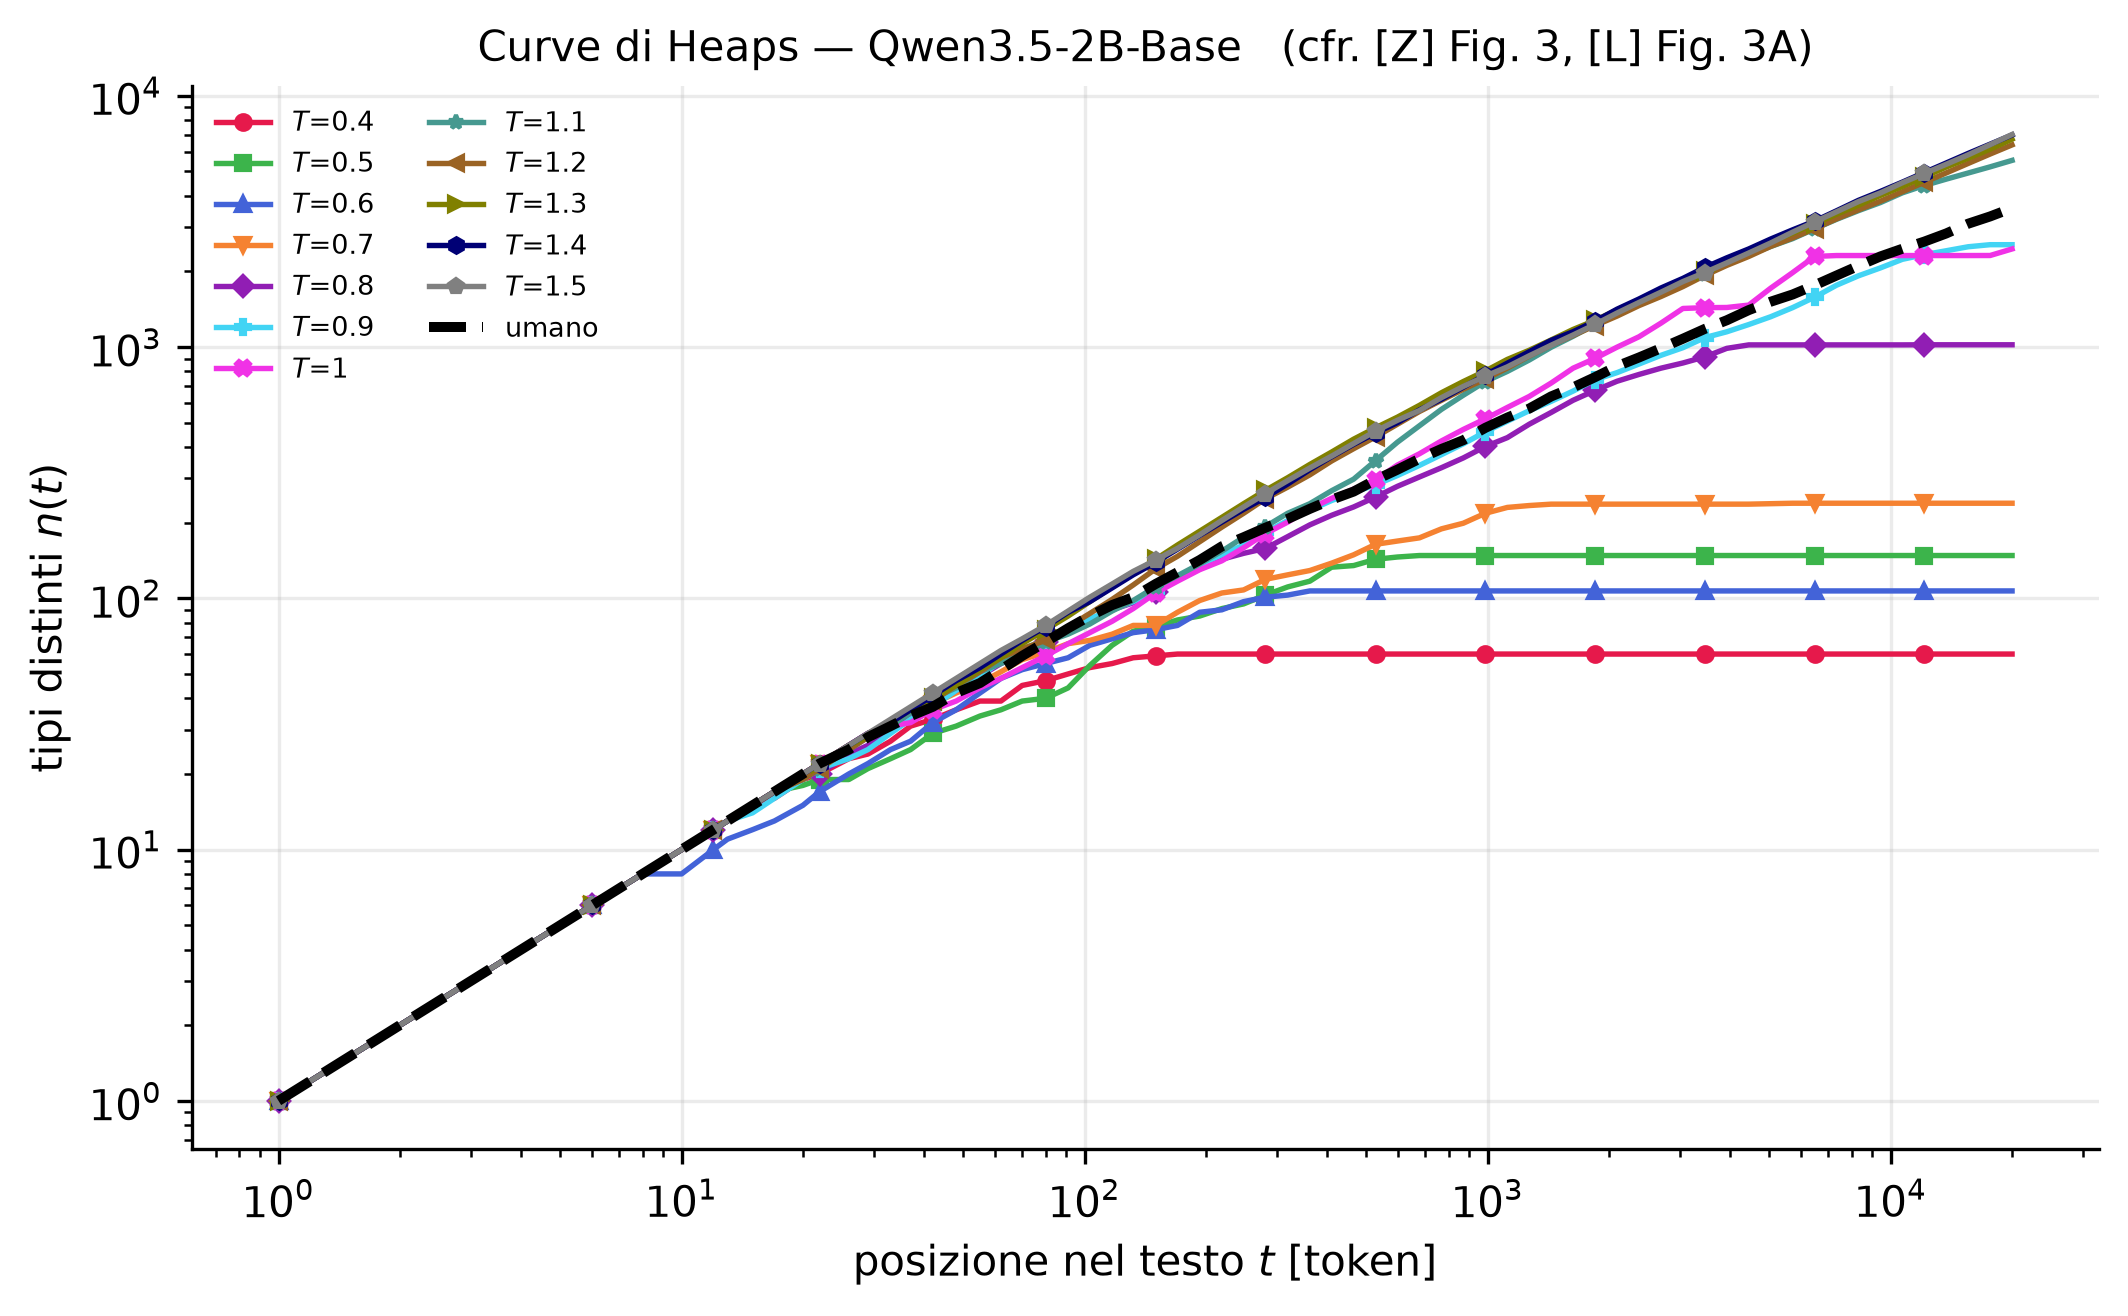
\includegraphics[width=0.56\textwidth]{figure/cap4_heaps_curve_Qwen35_2B_Base.png}
  \caption{Qwen3.5-2B-Base.}
\end{figure}

\begin{figure}[!htb]
  \centering
  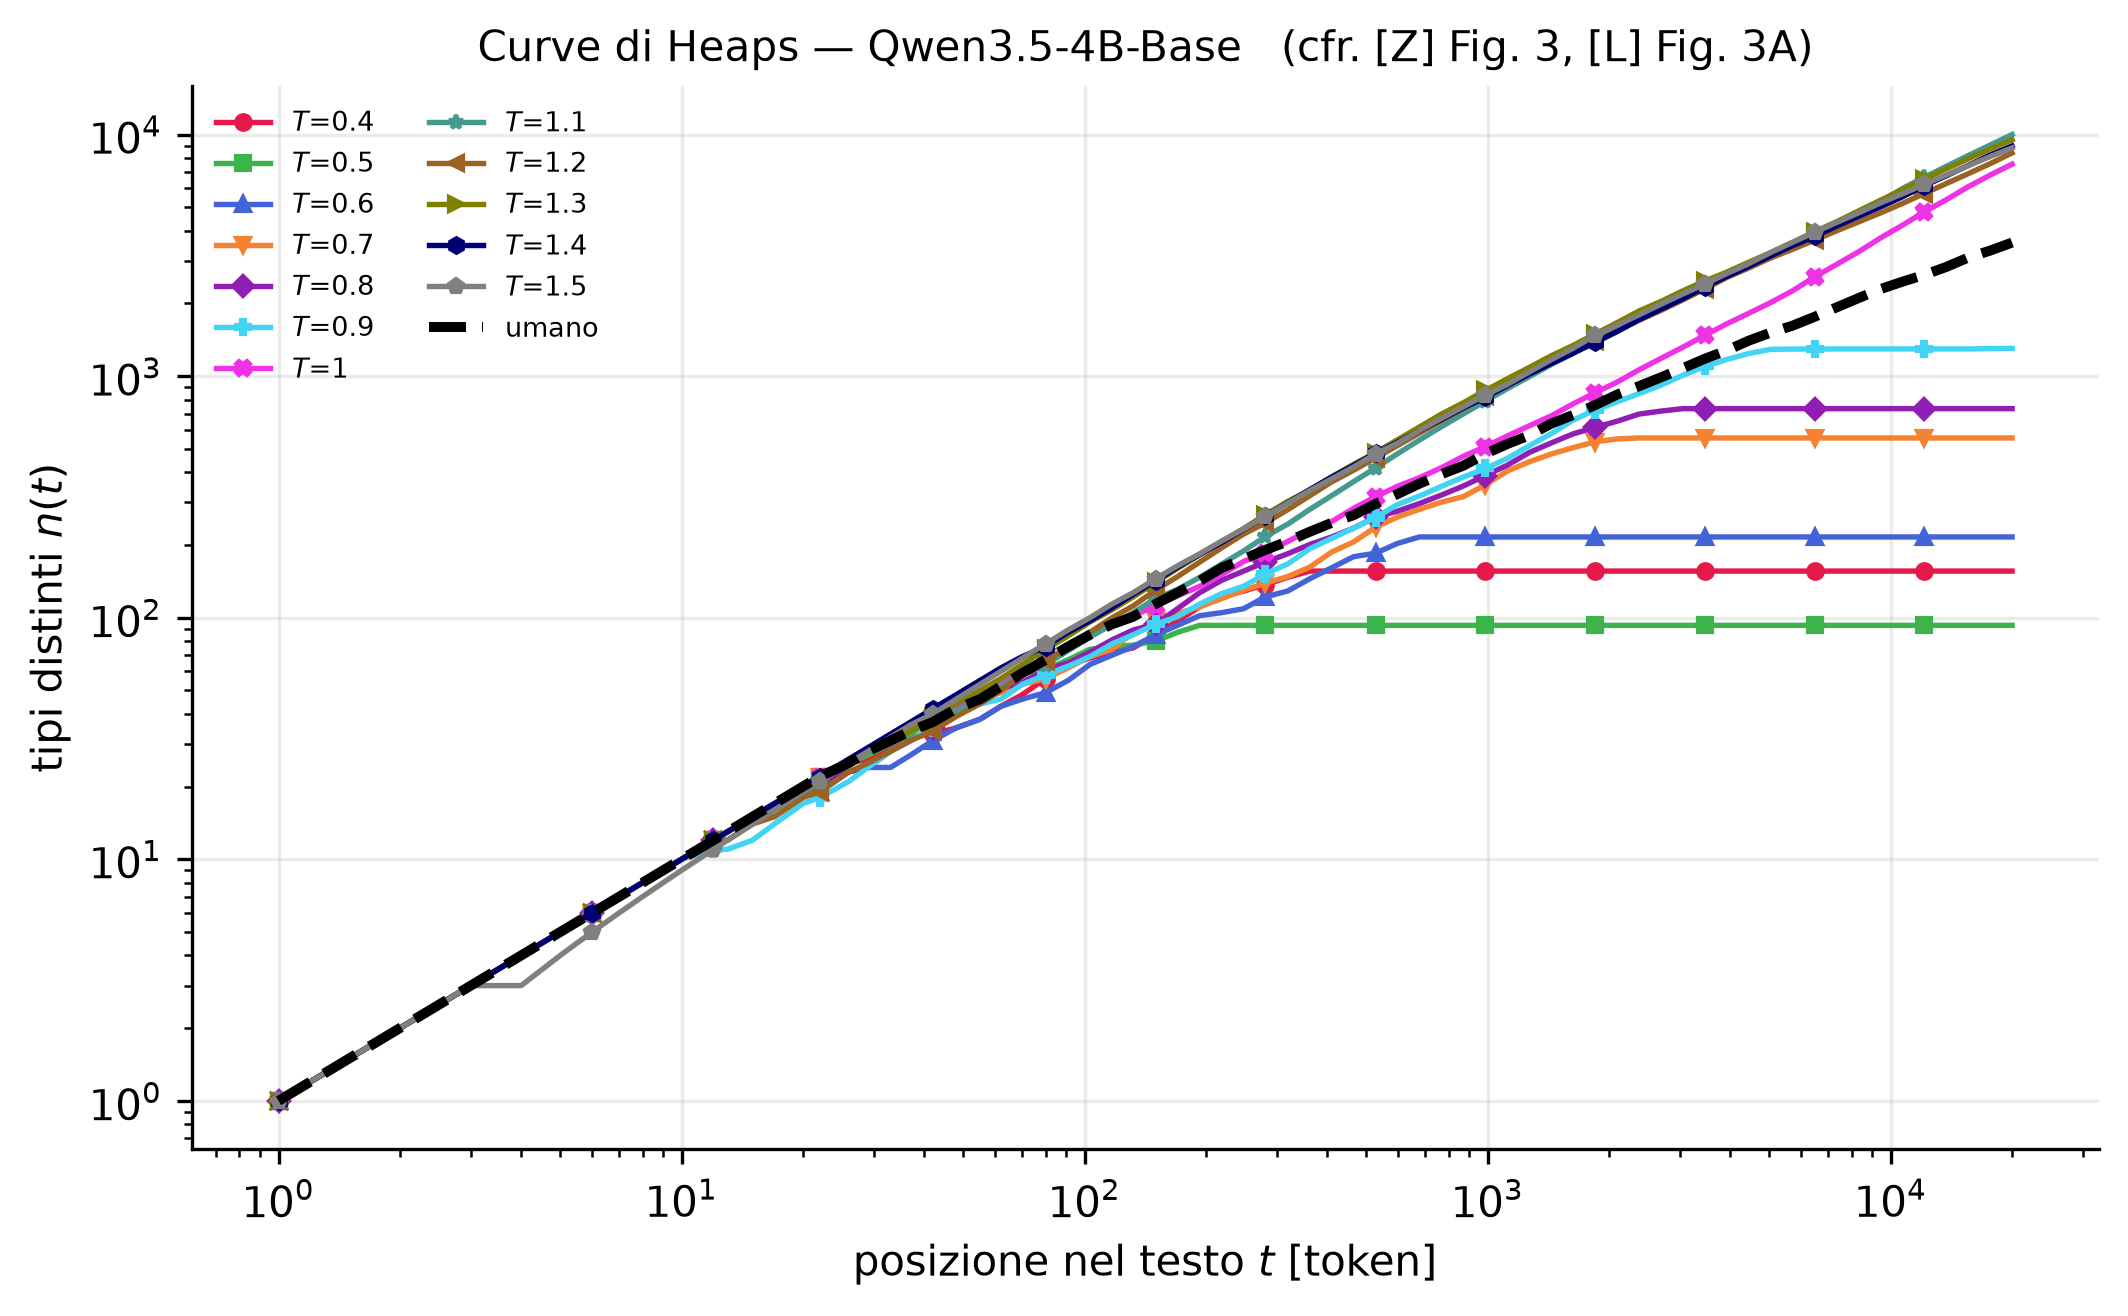
\includegraphics[width=0.56\textwidth]{figure/cap4_heaps_curve_Qwen35_4B_Base.png}
  \caption{Qwen3.5-4B-Base.}
\end{figure}

% ---------------------------------------------------------------------
\section{Fluttuazione detrendizzata}
\label{app:dfa}

\begin{figure}[!htb]
  \centering
  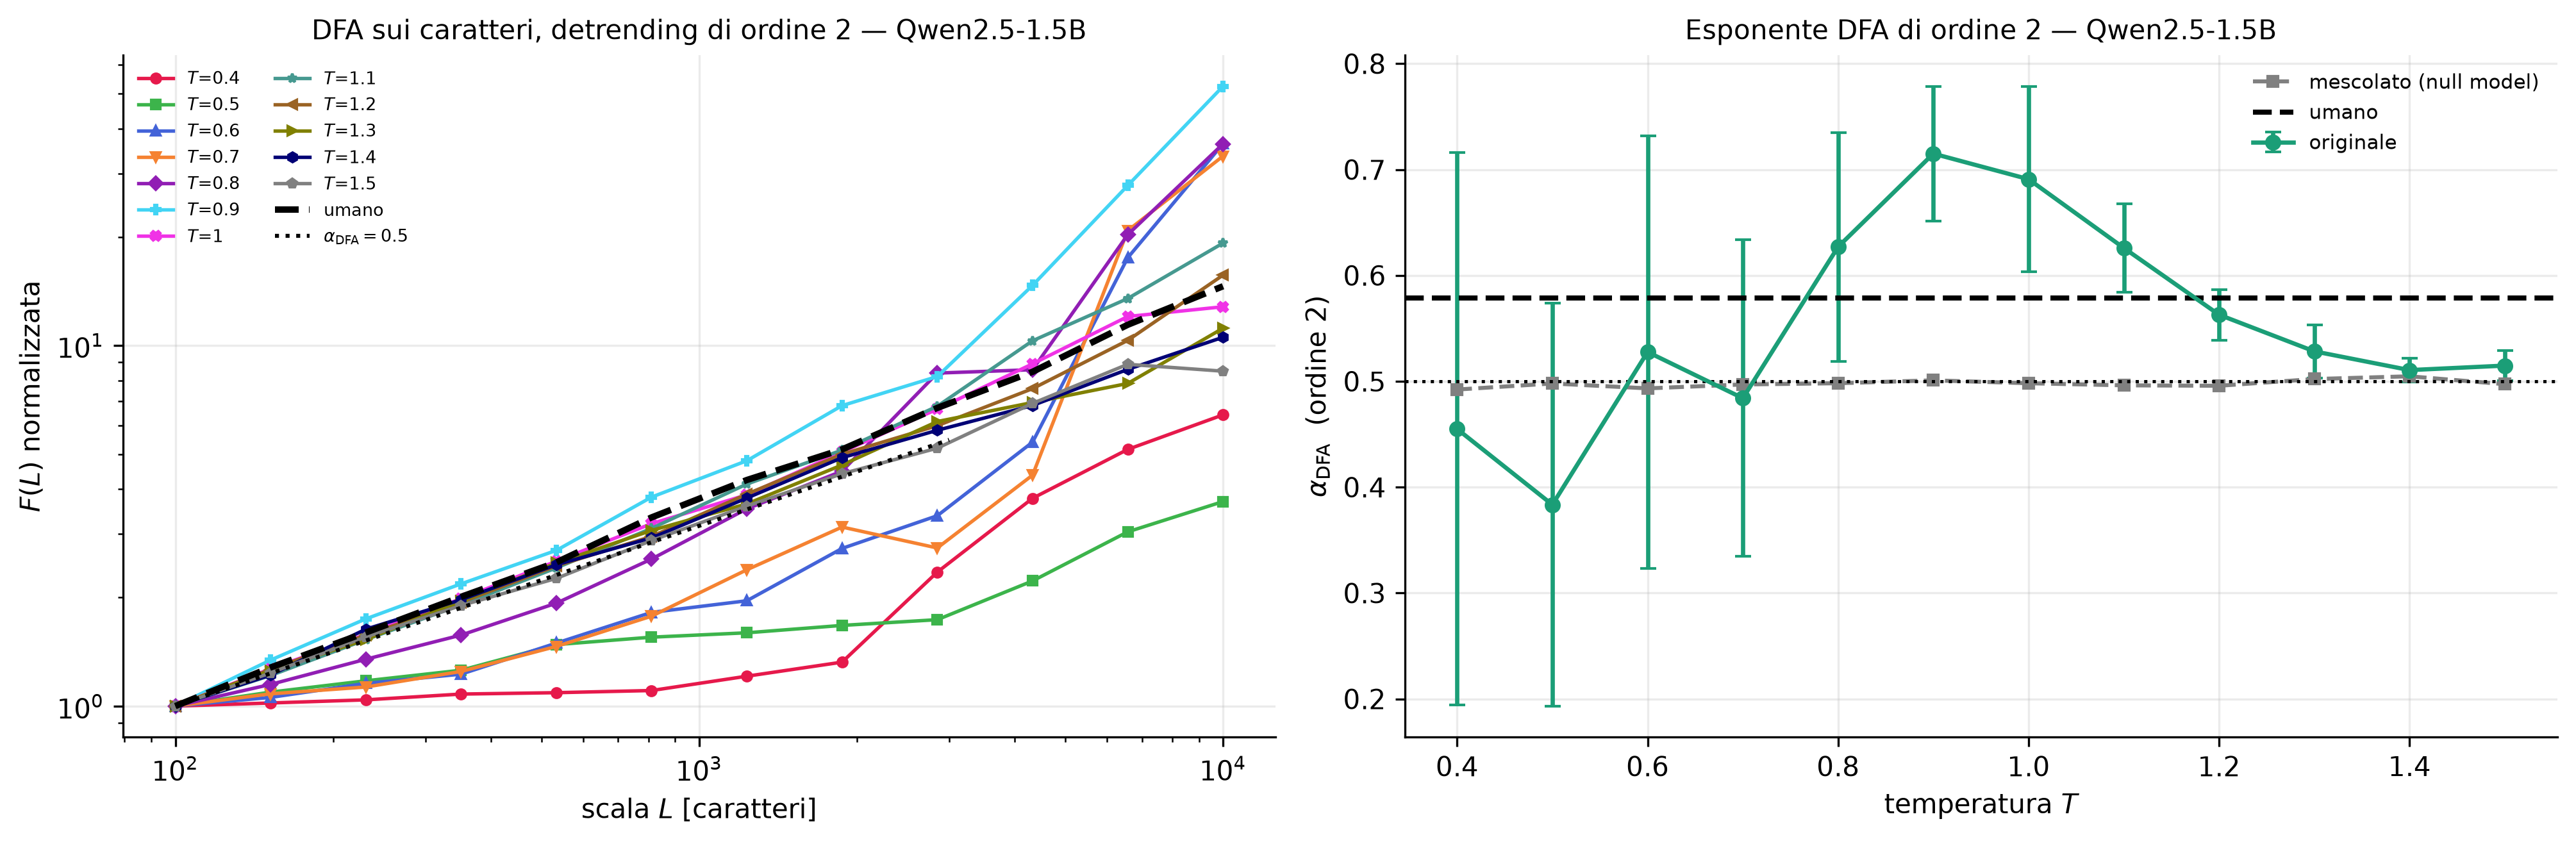
\includegraphics[width=0.80\textwidth]{figure/cap4_dfa_Qwen25_15B_o2.png}
  \caption{Qwen2.5-1.5B.}
\end{figure}

\begin{figure}[!htb]
  \centering
  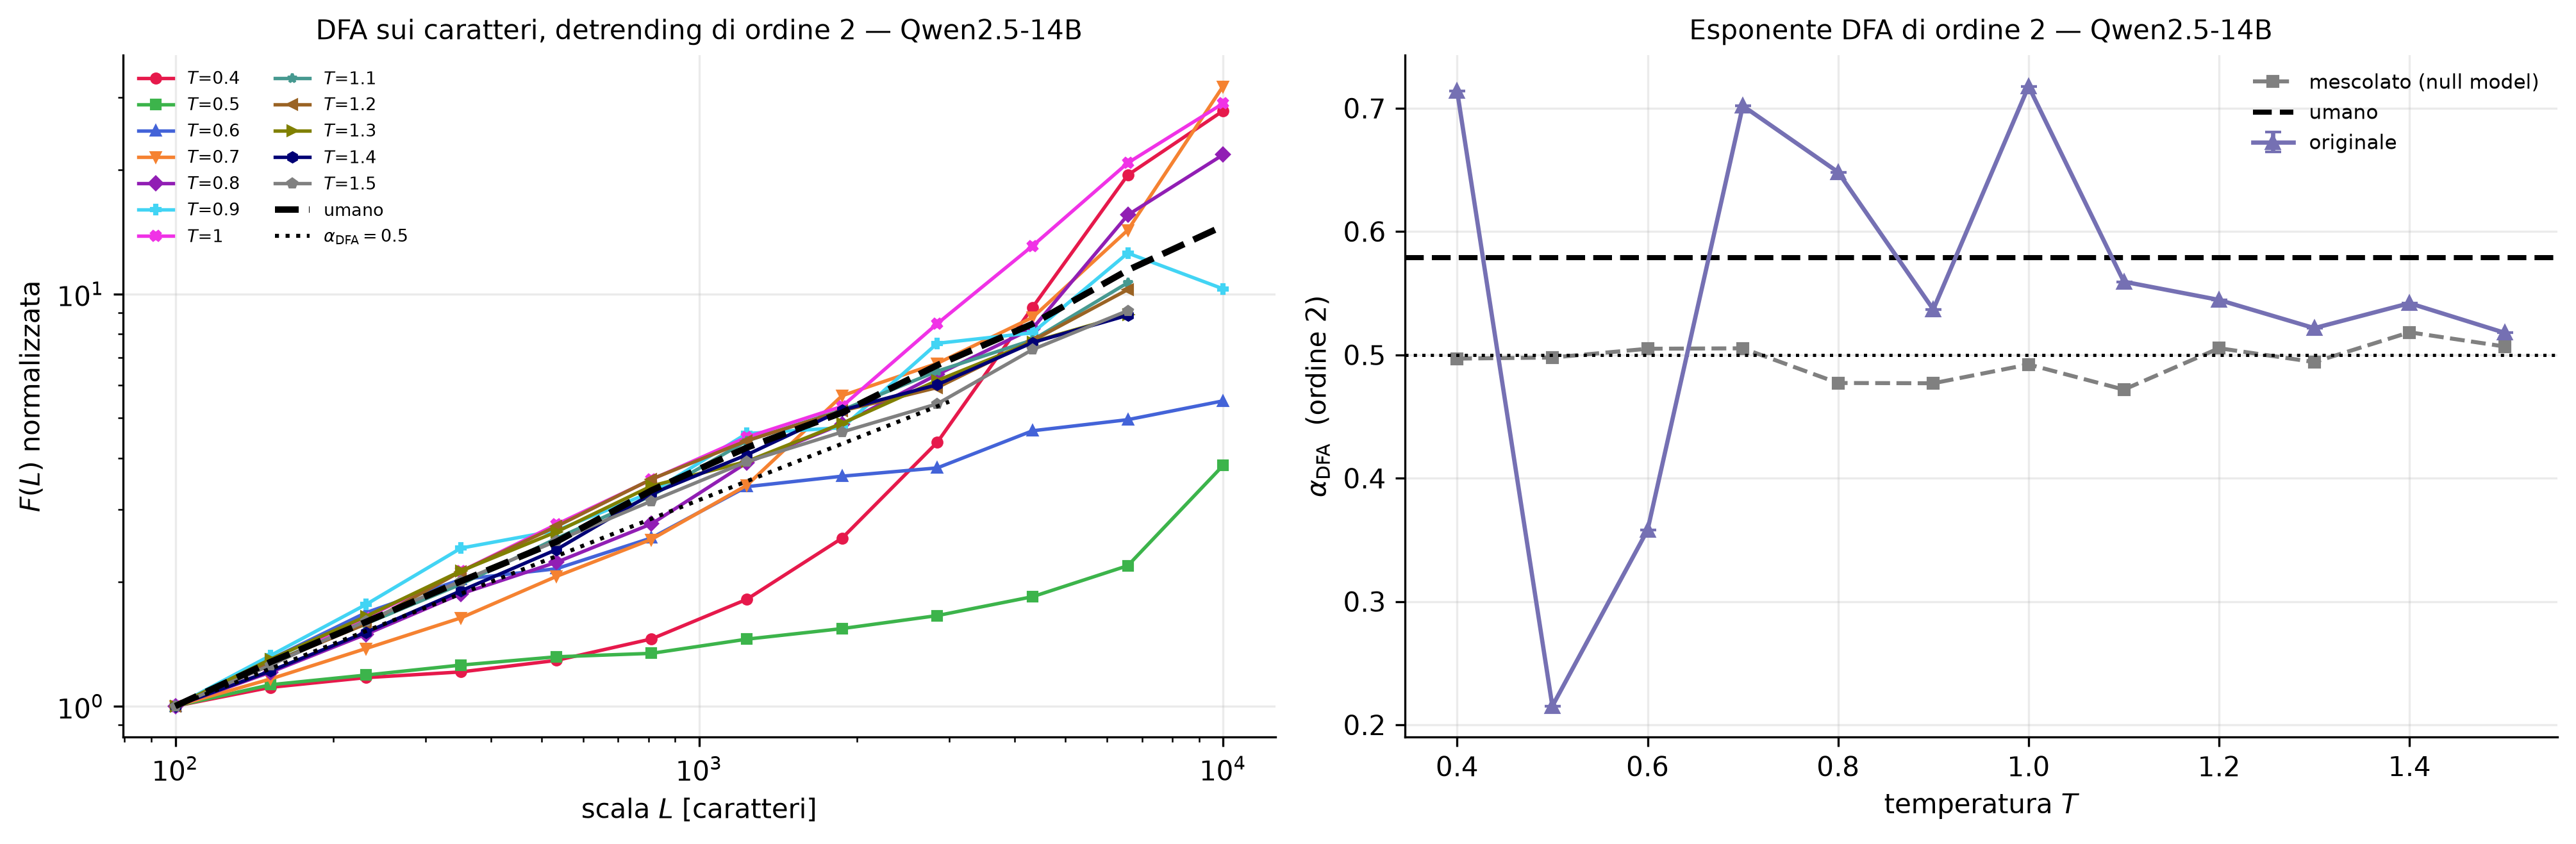
\includegraphics[width=0.80\textwidth]{figure/cap4_dfa_Qwen25_14B_o2.png}
  \caption{Qwen2.5-14B. Le barre d'errore non sono definite, poiché il modello
  dispone di un solo campione per temperatura.}
\end{figure}

\begin{figure}[!htb]
  \centering
  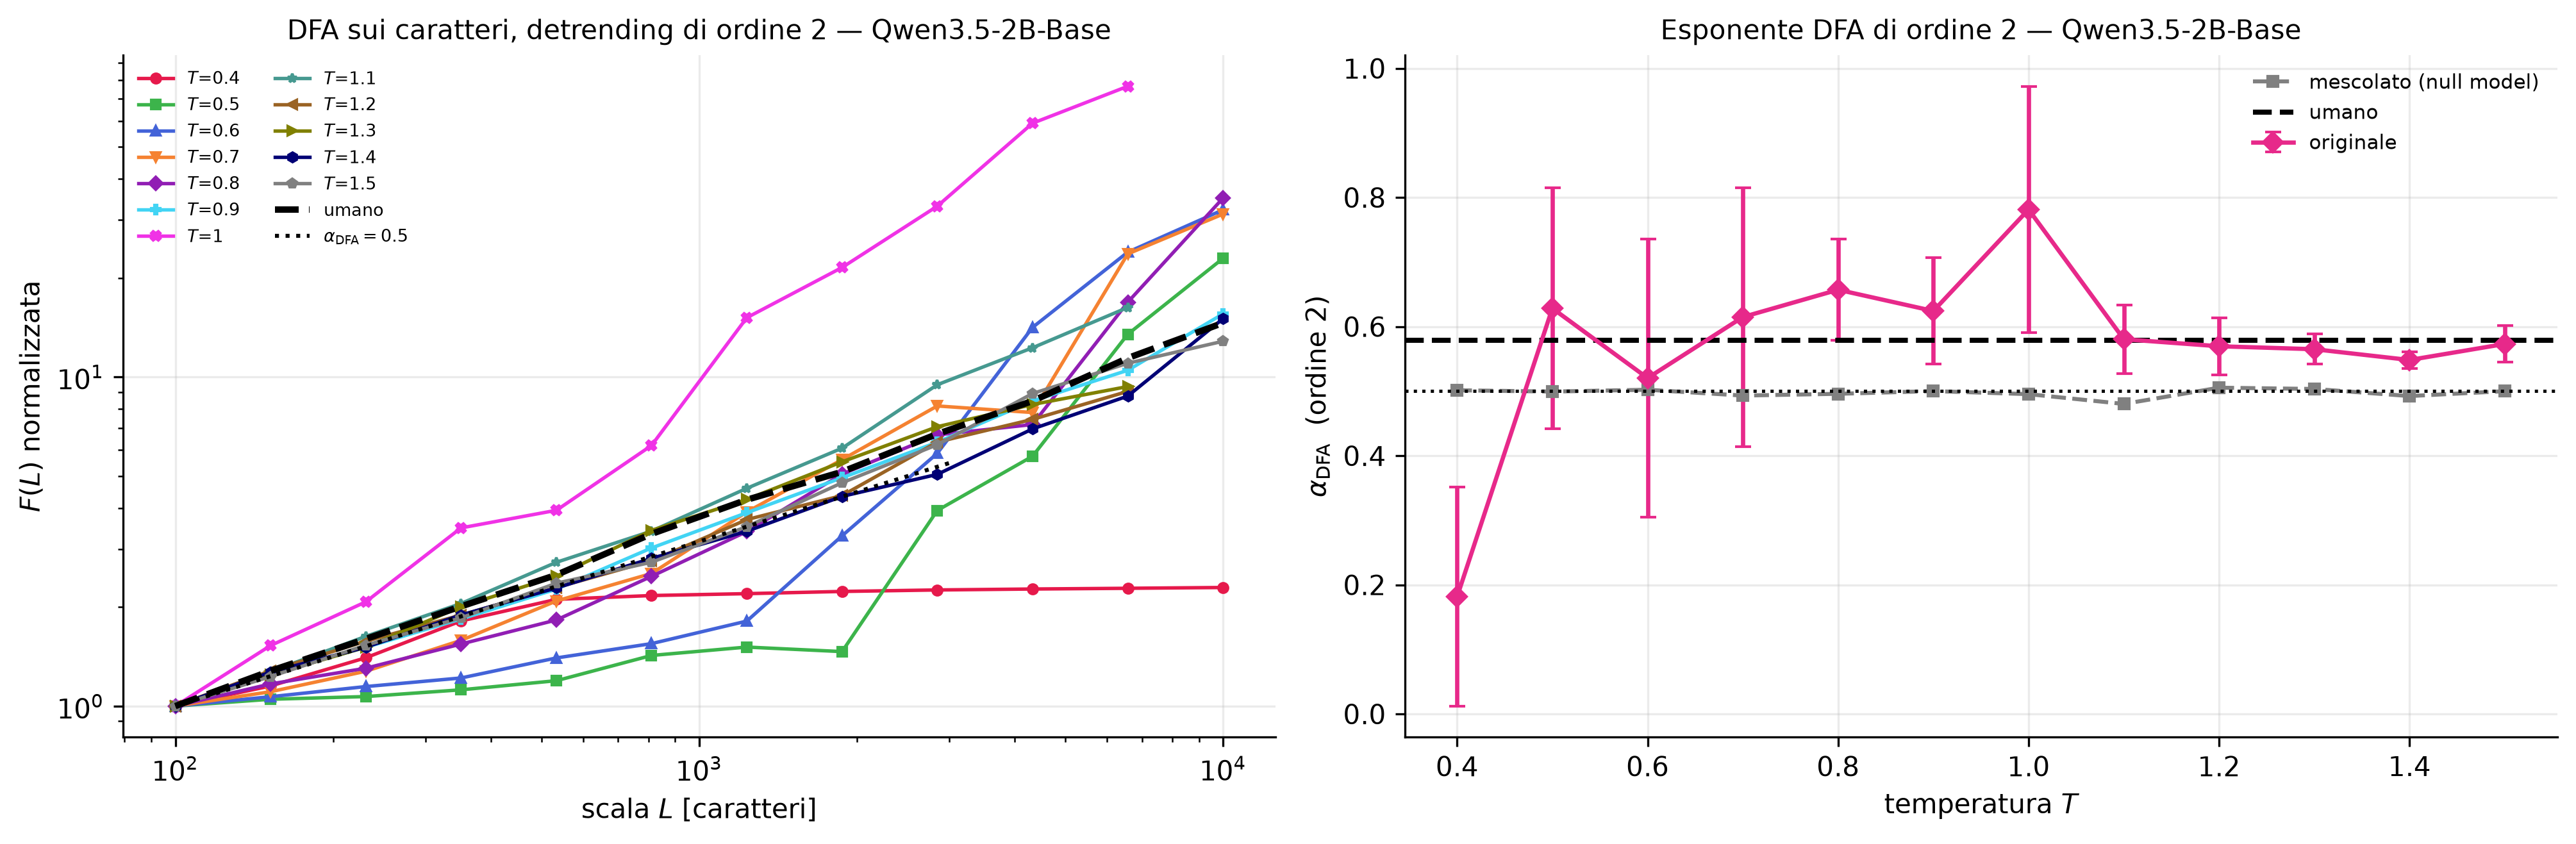
\includegraphics[width=0.80\textwidth]{figure/cap4_dfa_Qwen35_2B_Base_o2.png}
  \caption{Qwen3.5-2B-Base.}
\end{figure}

\begin{figure}[!htb]
  \centering
  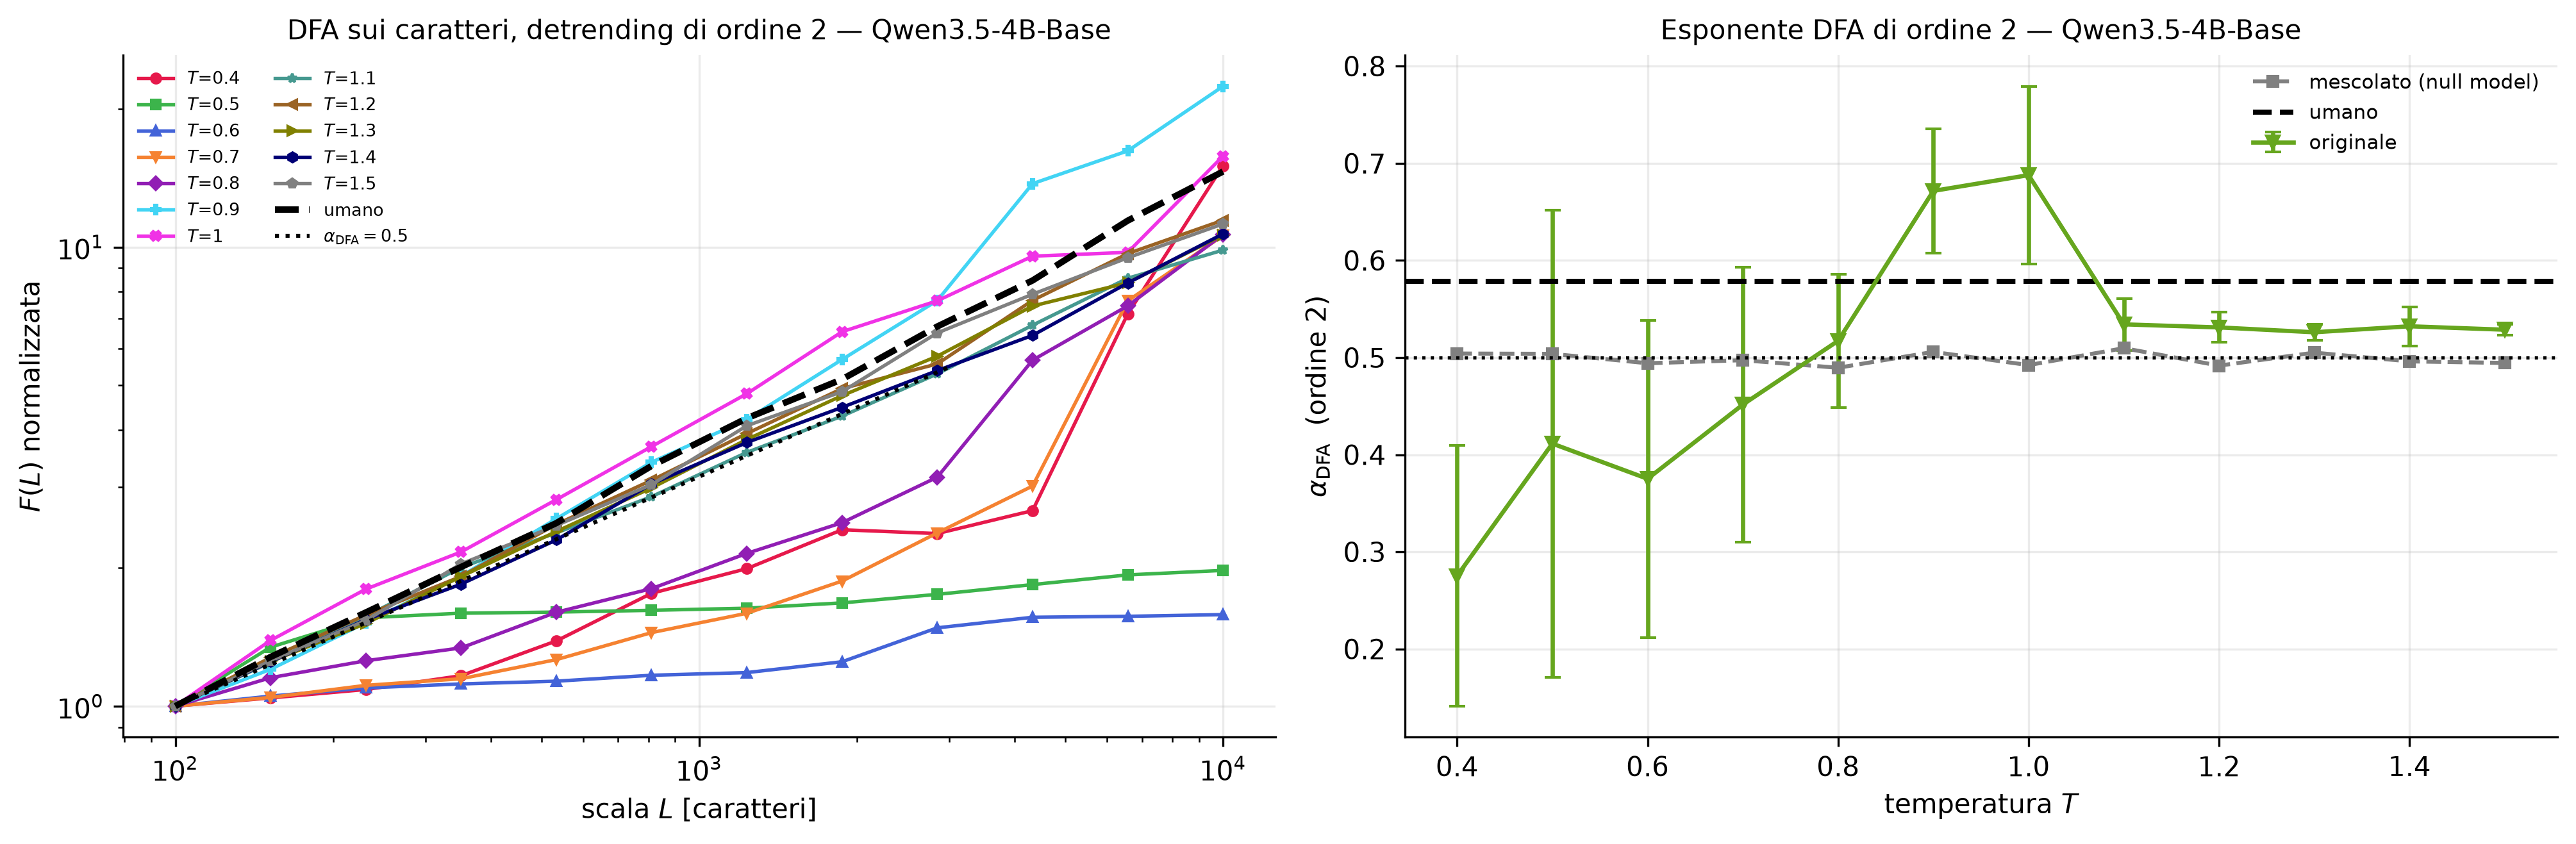
\includegraphics[width=0.80\textwidth]{figure/cap4_dfa_Qwen35_4B_Base_o2.png}
  \caption{Qwen3.5-4B-Base.}
\end{figure}

% ---------------------------------------------------------------------
\section{Autocorrelazione della traiettoria di embedding}
\label{app:acf}

\begin{figure}[!htb]
  \centering
  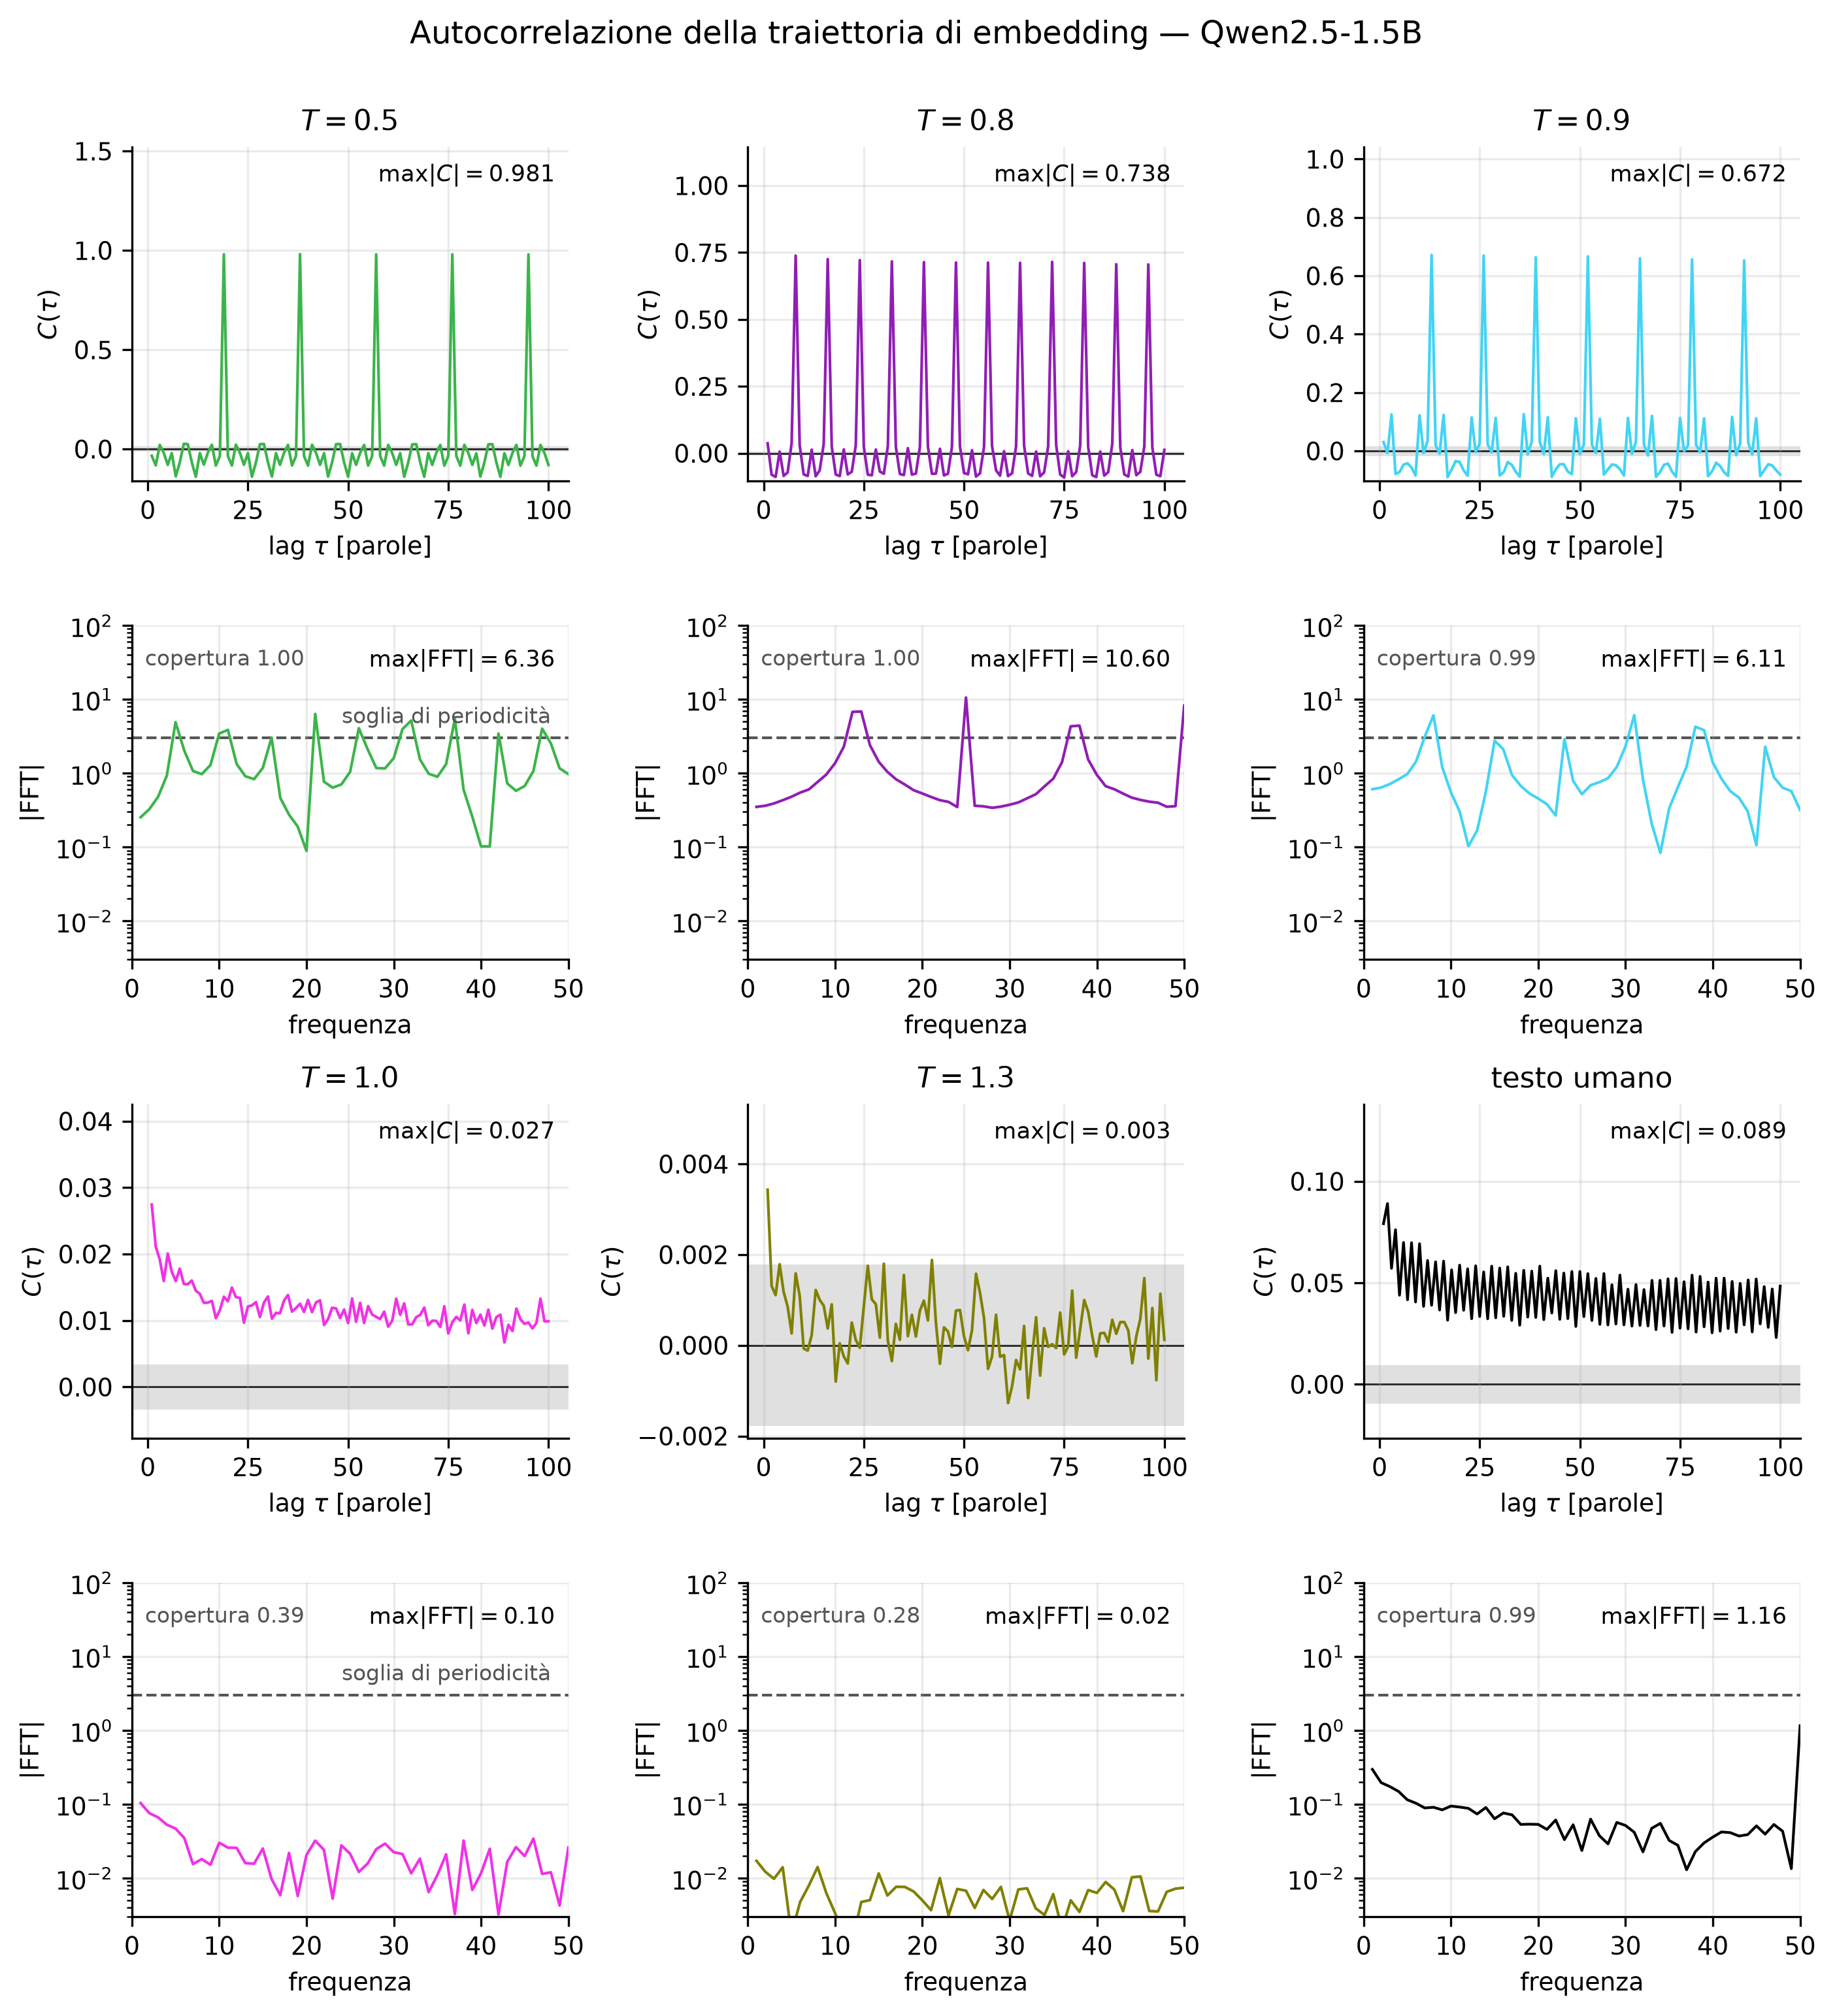
\includegraphics[width=0.58\textwidth]{figure/cap4_acf_Qwen25_15B.png}
  \caption{Qwen2.5-1.5B.}
\end{figure}

\begin{figure}[!htb]
  \centering
  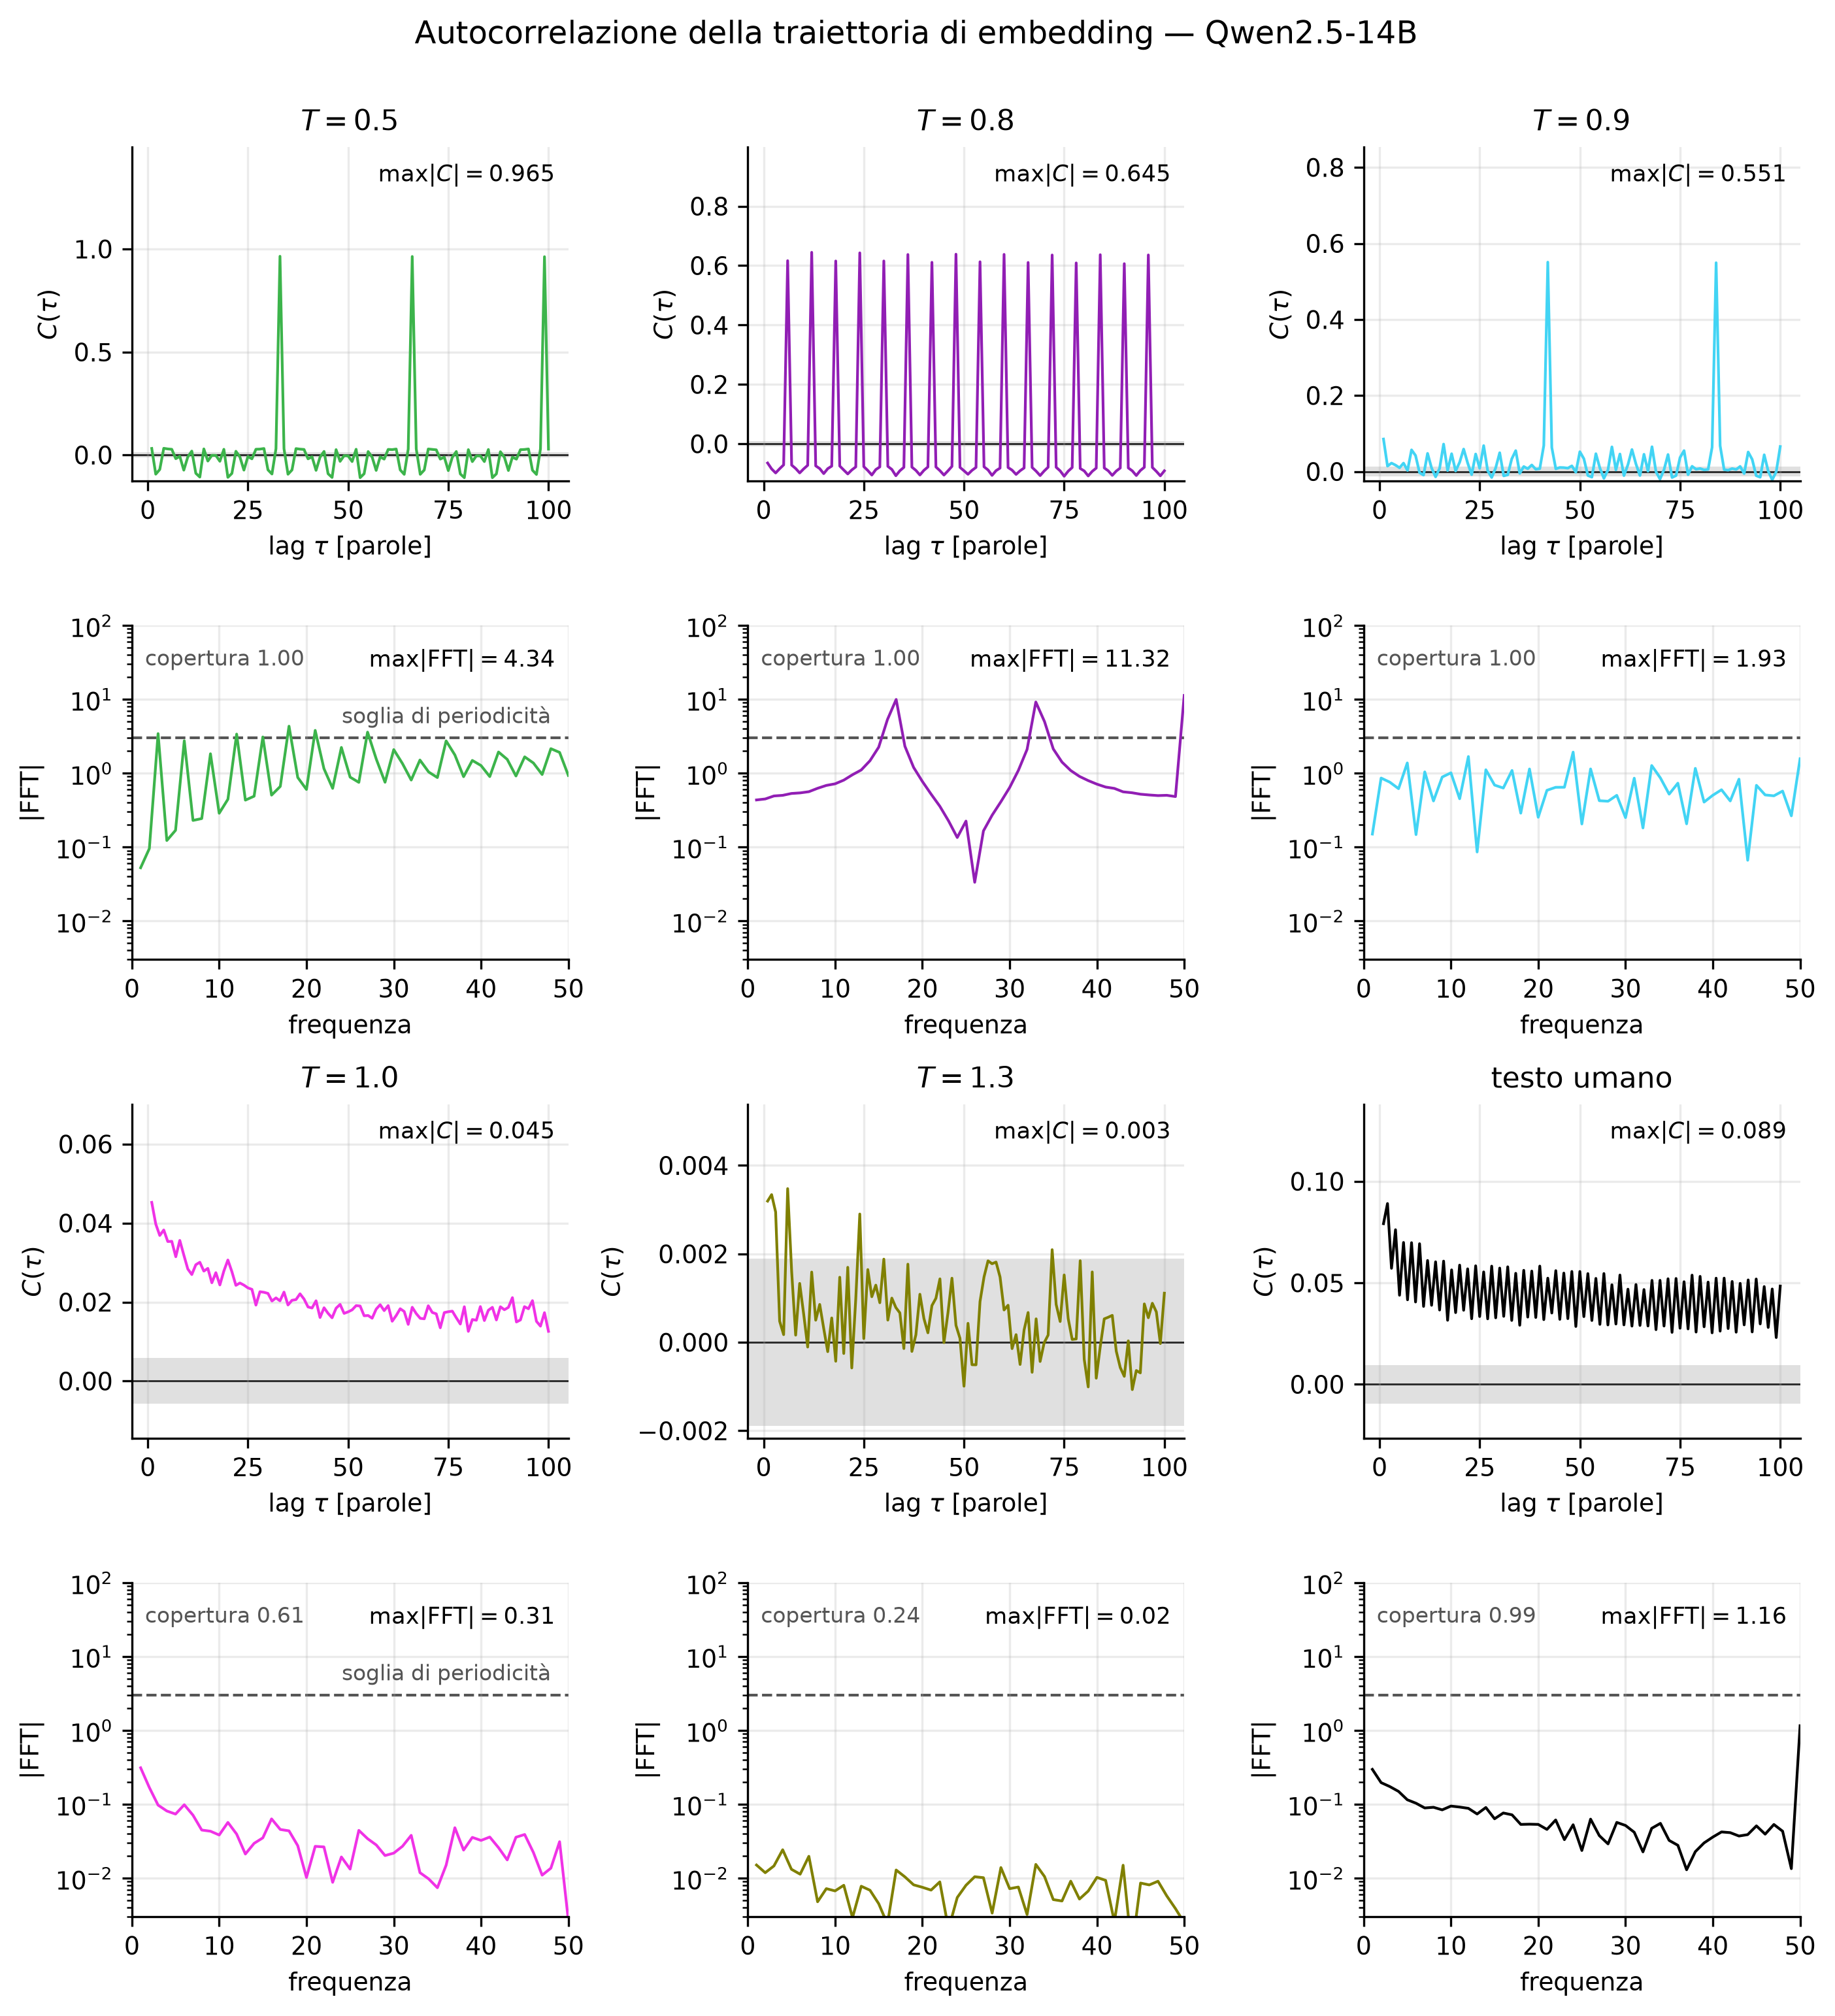
\includegraphics[width=0.58\textwidth]{figure/cap4_acf_Qwen25_14B.png}
  \caption{Qwen2.5-14B.}
\end{figure}

\begin{figure}[!htb]
  \centering
  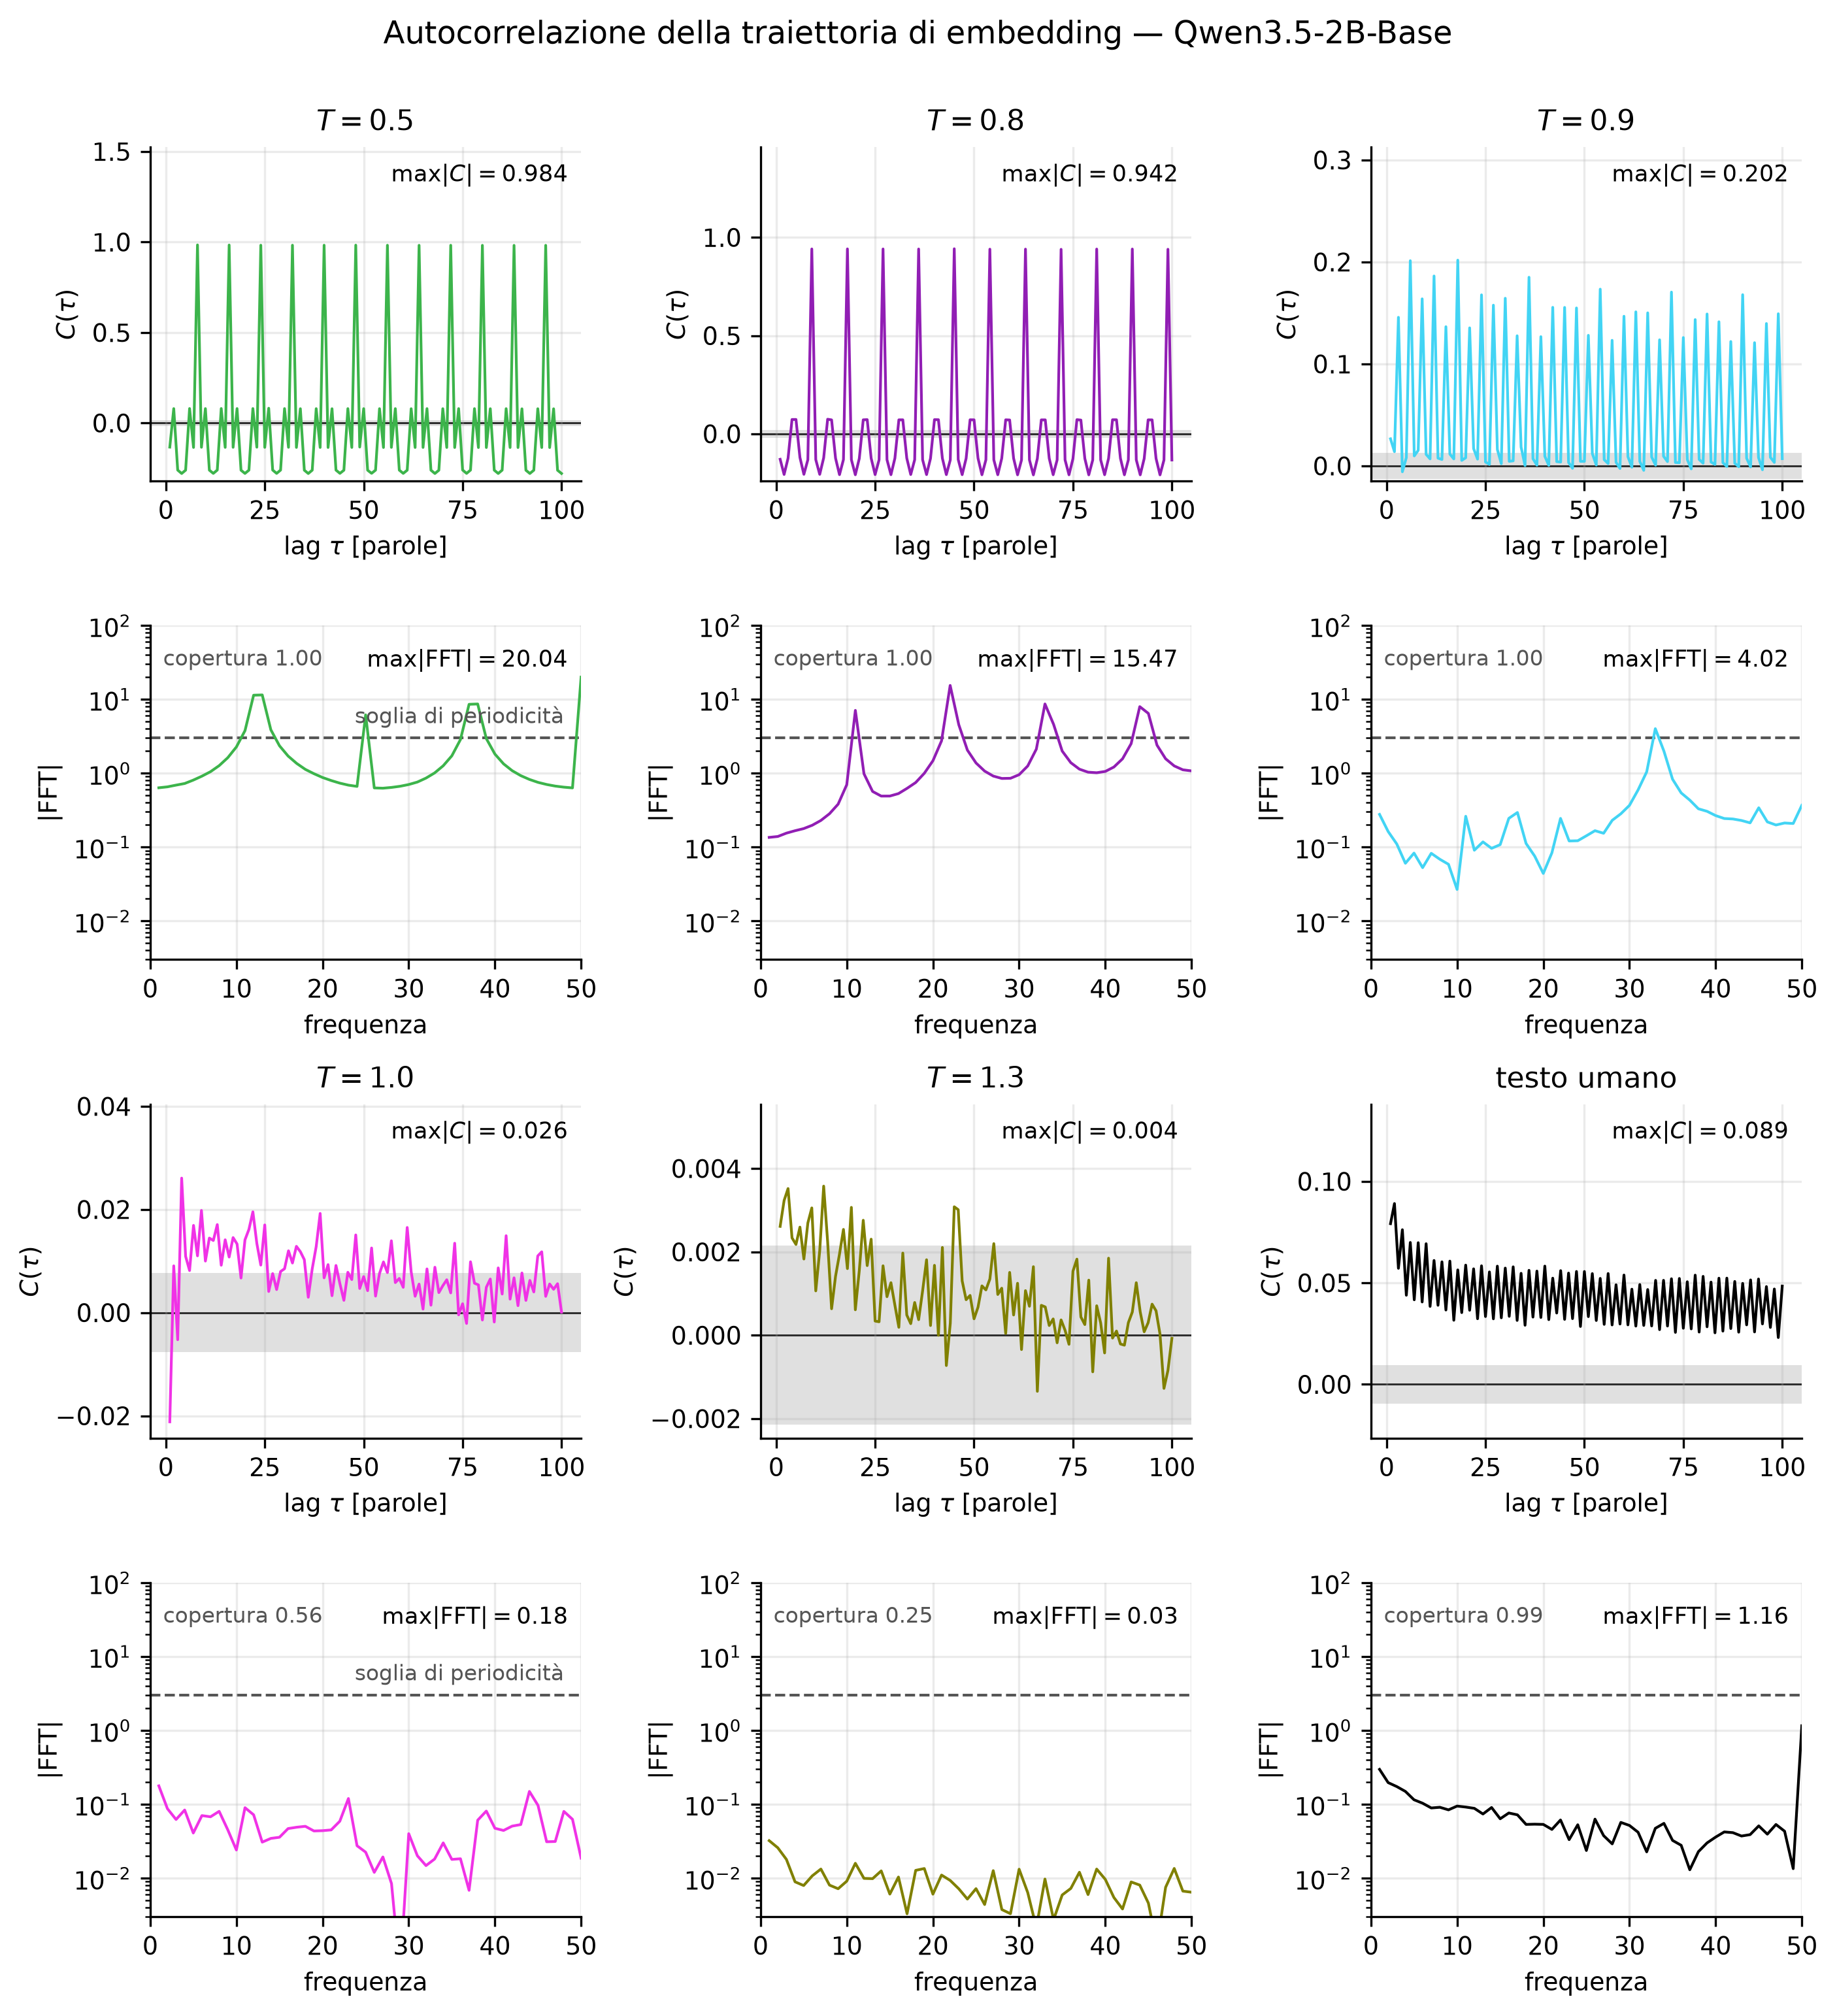
\includegraphics[width=0.58\textwidth]{figure/cap4_acf_Qwen35_2B_Base.png}
  \caption{Qwen3.5-2B-Base.}
\end{figure}

\begin{figure}[!htb]
  \centering
  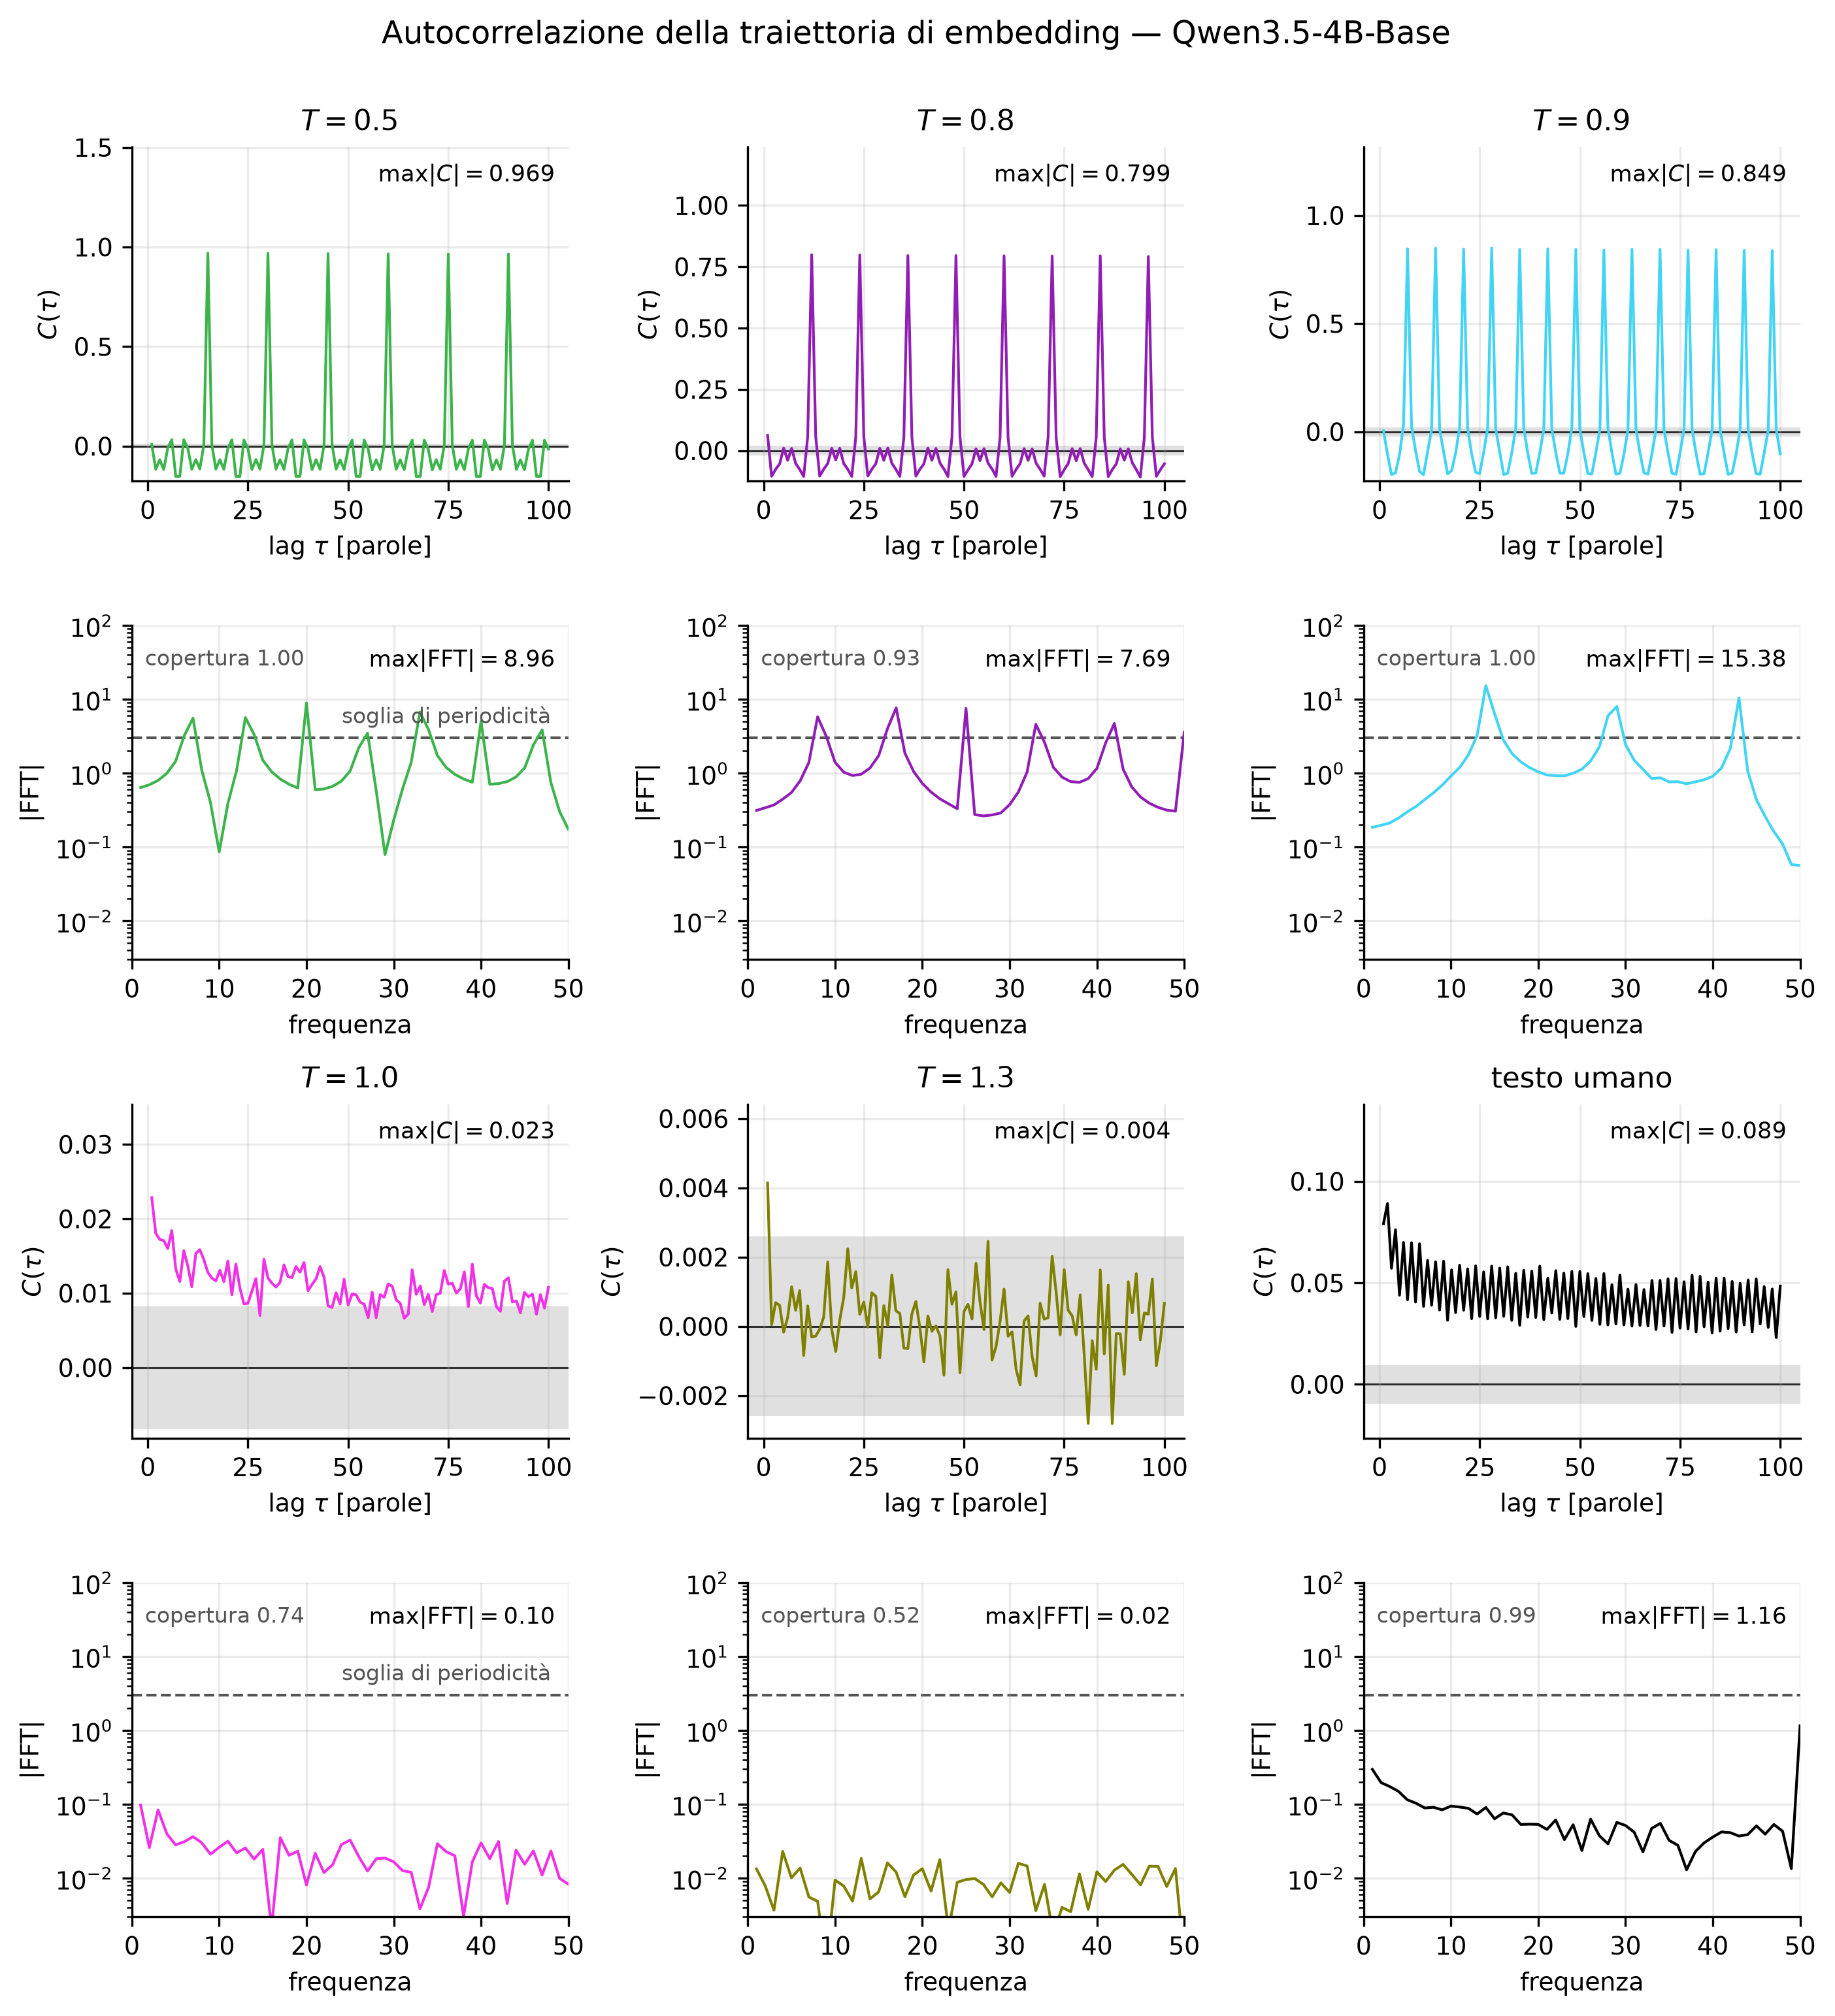
\includegraphics[width=0.58\textwidth]{figure/cap4_acf_Qwen35_4B_Base.png}
  \caption{Qwen3.5-4B-Base.}
\end{figure}
